\section{Confronto veicolo Ego Simulato e Reale}
In questa sezione verranno analizzati i dati del veicolo \emph{ego} simulato confrontandoli 
con i dati del veicolo \emph{ego} reale. L'obiettivo è valutare quanto il modello proposto si avvicini 
al comportamento di un sistema ACC reale disponibile in commercio.
\subsection{Accelerazione}
In Figura \ref{fig:acceleration_impartita} viene confrontata l'accelerazione del veicolo \emph{ego} simulato (in blu) 
con l'accelerazione impartita al veicolo \emph{ego} reale dal suo ACC (in giallo). 
\begin{figure}[H]
    \centering
    \adjustbox{center}{
        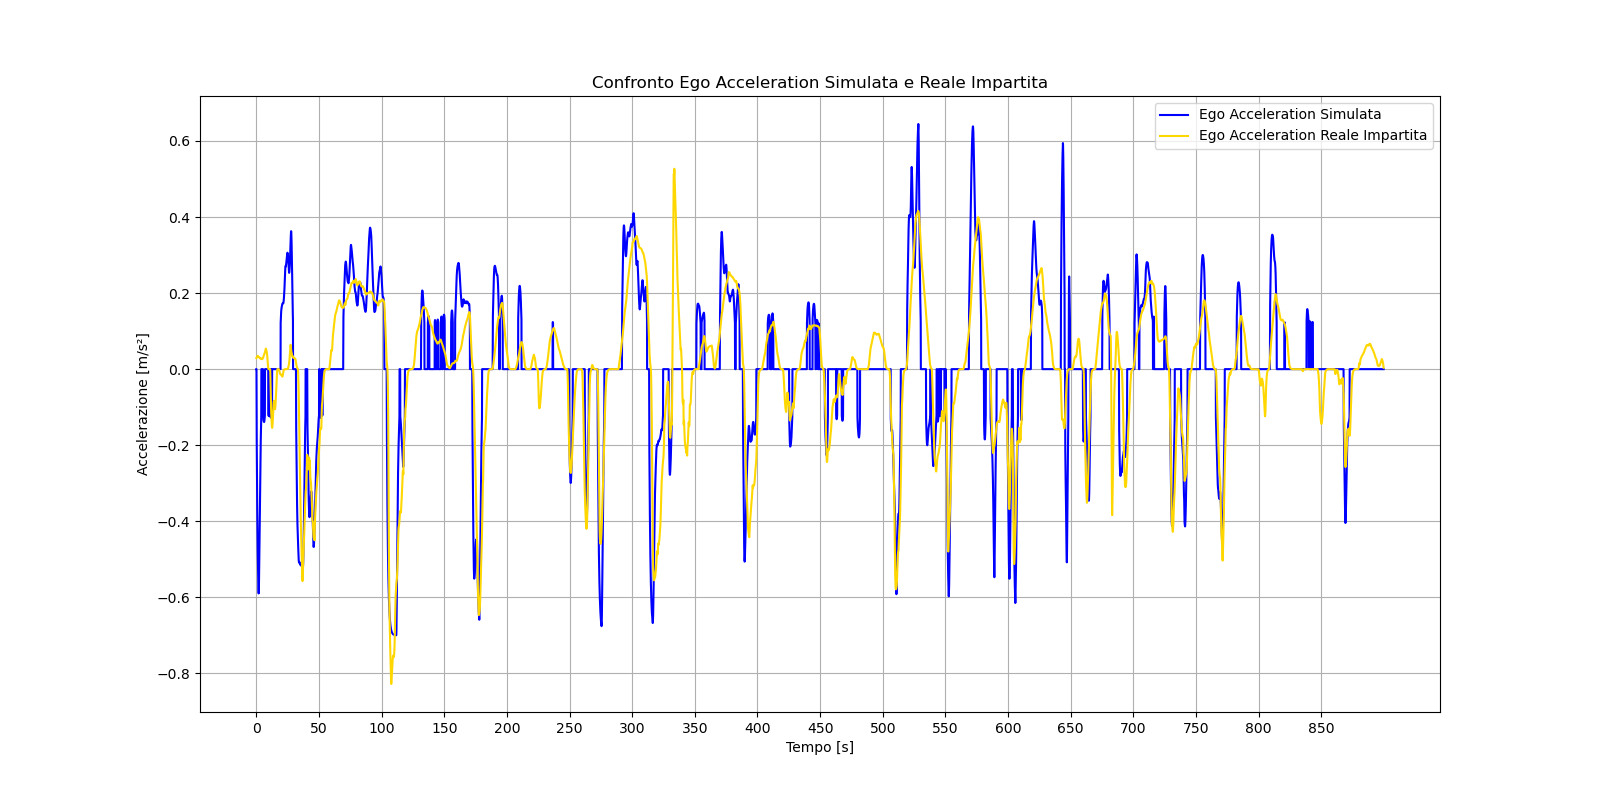
\includegraphics[width=1.25\linewidth]{simulation/real_data_comparison/acceleration_impartita.png}
    }
    \caption{Confronto Ego Acceleration Simulata e Reale Impartita}
    \label{fig:acceleration_impartita}
\end{figure}

\noindent La vicinanza delle due linee evidenzia come il modello proposto riproduca fedelmente il trend degli output di un ACC reale.  
I picchi e le valli delle due serie di dati si allineano, suggerendo che il modello è in grado di catturare 
non solo l'entità, ma anche il timing delle variazioni di accelerazione.  
\\\\
\noindent Il coefficiente di correlazione di Pearson pari a \textbf{0.771} conferma questa osservazione: un valore elevato indica 
una forte correlazione lineare positiva tra le due variabili.
\\\\
\noindent Questi risultati dimostrano che il modello di ACC proposto riproduca in modo realistico il comportamento 
di un sistema reale. Va tuttavia sottolineato che, essendo basato su dati del 2019, i sistemi ACC attuali potrebbero 
avere performance e strategie di controllo ancora più avanzate.
\\\\
\noindent In Figura \ref{fig:acceleration_effettiva} viene confrontata l'accelerazione del veicolo \emph{ego} simulato (in blu) 
con l'accelerazione effettiva al veicolo \emph{ego} reale (in viola). 
\begin{figure}[H]
    \centering
    \adjustbox{center}{
        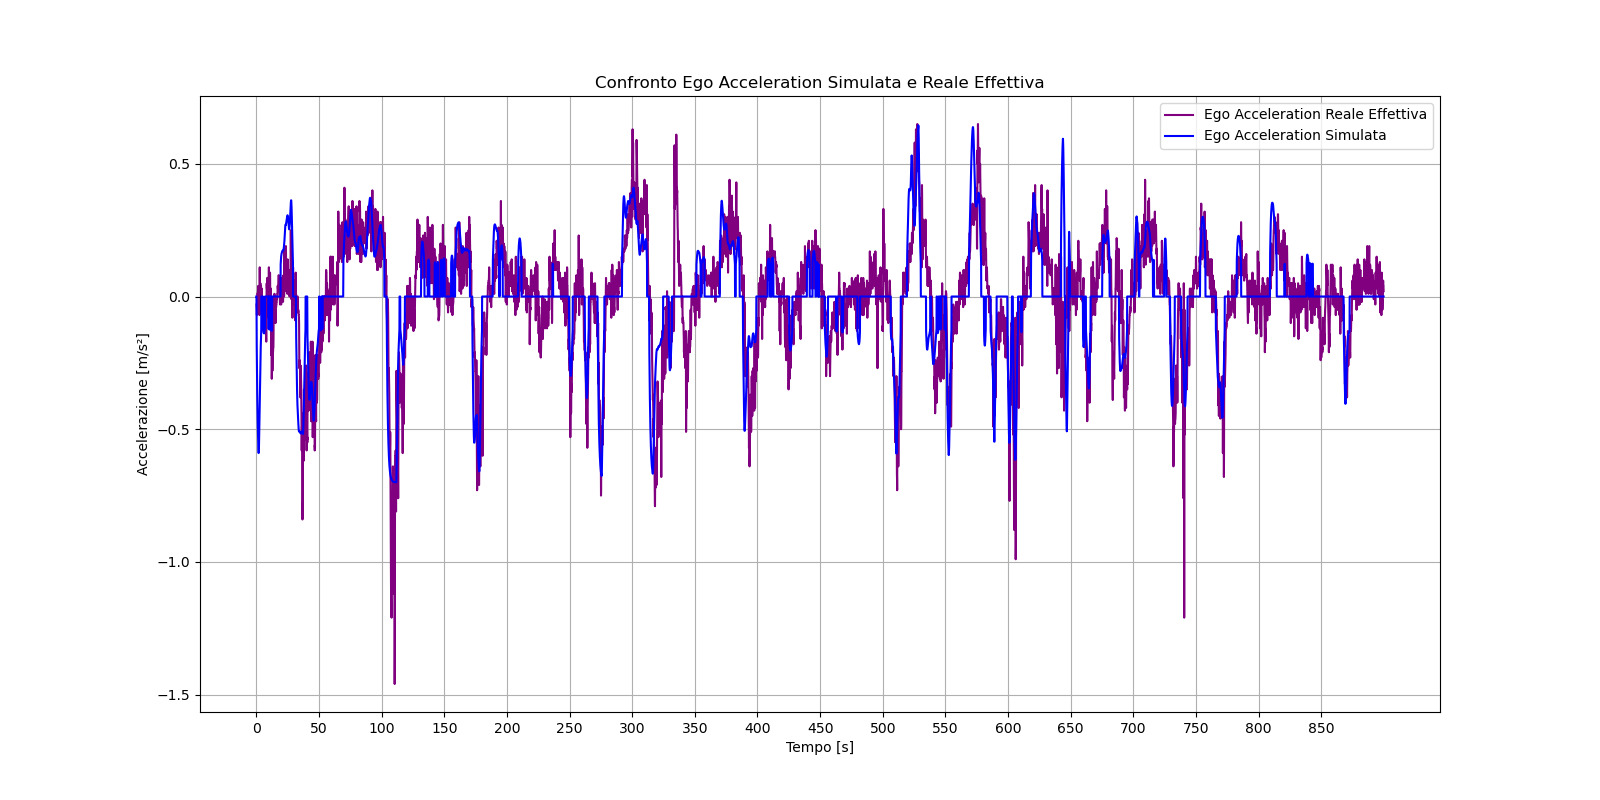
\includegraphics[width=1.25\linewidth]{simulation/real_data_comparison/acceleration_effettiva.png}
    }
    \caption{Confronto Ego Acceleration Simulata e Reale Effettiva}
    \label{fig:acceleration_effettiva}
\end{figure}
\noindent Questo confronto è stato effettuato in continuità con quanto discusso nella Sezione \ref{sec:premessa}.  
Anche in questo caso, l'accelerazione simulata segue il trend dell'accelerazione effettiva misurata sul veicolo reale.  
Il coefficiente di correlazione di Pearson risulta pari a \textbf{0.750}, leggermente inferiore al valore 0.771 osservato 
precedentemente. La differenza è dovuta al fatto che qui non si confrontano due sistemi ACC, ma l'ACC simulato con l'accelerazione 
effettiva del veicolo, che, come spiegato nella Sezione \ref{sec:premessa}, può discostarsi dall'accelerazione teoricamente 
impartita a causa delle dinamiche del veicolo.

\subsection{Velocità}
\noindent In Figura \ref{fig:ego_velocity_reale} viene confrontata la velocità del veicolo \emph{ego} simulato (in blu) 
con la velocità del veicolo \emph{ego} reale (in giallo). 
\begin{figure}[H]
    \centering
    \adjustbox{center}{
        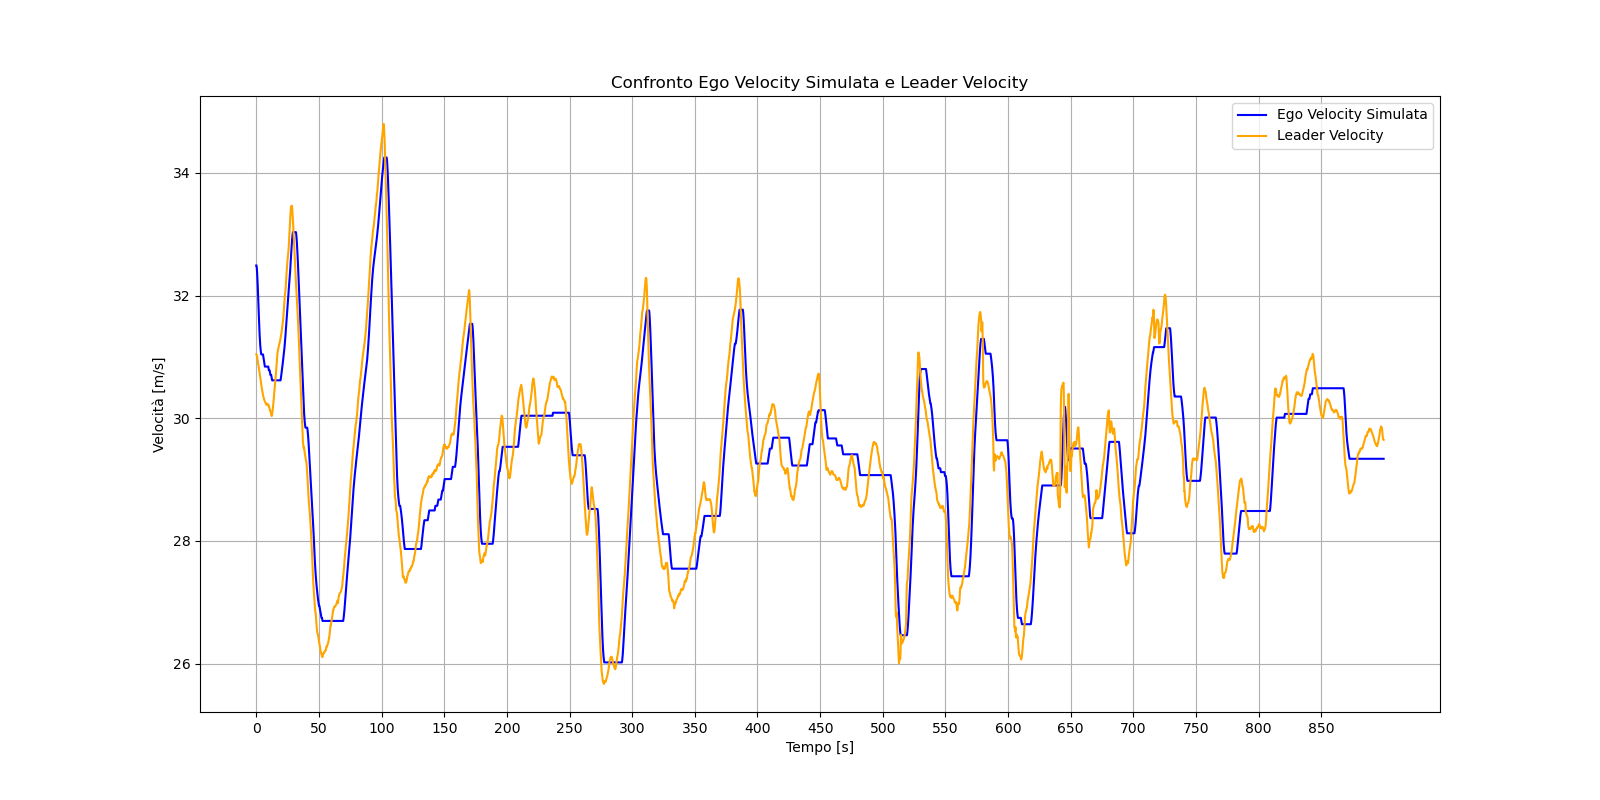
\includegraphics[width=1.25\linewidth]{simulation/real_data_comparison/velocity.png}
    }
    \caption{Confronto Ego Velocity Simulata e Reale}
    \label{fig:ego_velocity_reale}
\end{figure}
\noindent Come osservato per le accelerazioni, la velocità simulata riproduce in modo fedele la dinamica della velocità reale.  
\\\\
\noindent Si evidenziano tuttavia alcune differenze: la curva simulata presenta talvolta sezioni piatte o “scalini”, 
dovuti alla definizione delle membership function per l'accelerazione e alla condizione che annulla qualsiasi 
accelerazione superiore a $0.12 \,\frac{\mathrm{m}}{\mathrm{s^2}}$ in modulo.
Tuttavia, la velocità reale risulta più irregolare e rumorosa, mentre quella simulata appare più smussata in alcuni tratti.  
\\\\
\noindent Nonostante queste piccole discrepanze, l'elevata corrispondenza tra le due curve è confermata dal coefficiente di 
correlazione di Pearson, pari a \textbf{0.957}.
